%=================================================================
\section{Problem Definition}\label{sec-intro}
%\todo{Narrow down to a topic; Dig a hole; Fill the hole}
The source of data for forecasting traffic flows in metropolitan areas in the USA is mainly based on kaggle competitions. The data contains characteristics such as time, coordinates, direction, etc. The aim of the article is to predict the amount of congestion at a particular time.\par 
The files and data attrubitions are described in Table 1:
\begin{center}
	\begin{table}[htbp]
		\setlength{\abovecaptionskip}{2pt}
		\centering
		\caption{DATA}
		\begin{tabular}{ c | c | c }
			\toprule
			% after \\: \hline or \cline{col1-col2} \cline{col3-col4} ...
			File    &Description      & Attribution       \\
			\midrule
			train.csv       &  \makecell{traffic congestion from April\\through September of 1991}   &  \makecell{row_id,time,x,y,\\direction,congestion}       \\
			\midrule
			test.csv       & \makecell{hourly predictions \\on the day of 1991-09-30}   &\makecell{row_id,time,x,y,\\direction}     \\
			\bottomrule
		\end{tabular}
	\end{table}
\end{center}



%\gangli{``narrow in on topic'' reminds you 
%that readers and reviewers only know that this is a AI or HTM research paper (and maybe have read the title/abstract). 
%You need to help them figure out what topic and area of research paper this is. 
%You _don't_ need to wax poetic about the topic's importance.}

%\gangli{`dig a hole'' reminds you that 
%you need to convince the reader that there's a problem with the state of the world. 
%Prior work may exist but it's either missing something important or there's a missing opportunity. 
%The reader should be drooling for a bright future just out of reach.}

%\gangli{``fill the hole'' reminds you to show the reader 
%how and why the paper they're reading will fix these problems and deliver us into a better place. 
%You don't need a whirlwind summary of the technical details, 
%but you need readers convinced (and in a good mood) to keep reading.}

%\todo{The importance of the area}
%\blindtext


\section{Data Processing} \label{sec-dataprocess}
Since the training data has both segmentable and mergeable data, we segmented the temporal data and merged the x, y and direction data.\par
First, we divide the 24 hours into 6 time periods, as in Table 2:
\begin{center}
	\begin{table}[htbp]
		\setlength{\abovecaptionskip}{2pt}
		\caption{period}
		\begin{tabular}{ c | c | c | c }
			\toprule
			period    &Description   &  period    &Description      \\
			\midrule
			Late Night     & 0:00-4:00 & Noon     & 12:00-16:00 \\
			\midrule
			Early Morning     & 4:00-8:00 & Evening     & 16:00-20:00 \\
			\midrule
			Morning     & 8:00-12:00 &  Night     & 20:00-24:00 \\
			\bottomrule
		\end{tabular}
	\end{table}
\end{center}\par
Second, we split the time into the following features:
\begin{itemize}
	\setlength{\itemsep}{-0.9ex} 
	\item
	\smallskip  
	month
	\item
	\smallskip
	weekday
	\item
	\smallskip
	minute
	\item
	\smallskip
	is_month_start
	\item
	\smallskip
	is_month_end
	\item
	\smallskip
	is_weekday
	\item
	\smallskip
	is_Monday
	\item
	\smallskip
	is_Friday
	\item
	\smallskip
	period
	\item
	\smallskip
	road:x+y+direction(00EB)
\end{itemize}



\section{Data Description} \label{datadescription}
After the data has been processed, the data is explored for congestion, time, road, etc. to find more potential relationships between them.\par
Firstly, the histogram(figure 1) shows the congestion data, which is normalised as can be seen from the graph.\par
Secondly, we use various graphs to show the relationship between features and congestion.(fig.2-fig.9)
\begin{figure}
	\setlength{\abovecaptionskip}{-0.1cm} 
	\includegraphics[width=10cm]{figure/congestion.eps}\\	
	\caption{Congestion data}
	\label{Congestion data}
\end{figure}

\begin{center}
	\begin{figure}[h]
		\setlength{\abovecaptionskip}{-0.1cm} 
		\includegraphics[width=10cm]{figure/weekday.eps}\\	
		\caption{The effect of weekday on congestion}
		\label{weekday}
	\end{figure}
\end{center}

\begin{center}
	
	\begin{figure}[htp]
	\setlength{\abovecaptionskip}{0.1cm} 
	\raggedleft
	\includegraphics[width=10cm]{figure/is_weekend.eps}
	\centering
	\caption{Congestion in special day or not}
	\label{special}
	\end{figure}
\end{center}

\begin{center}
	\begin{figure}[htp]
		\setlength{\abovecaptionskip}{0.1cm} 
		\raggedleft
		\includegraphics[width=10cm]{figure/is_weekend.eps}
		\centering
		\caption{Congestion in special day or not}
		\label{special}
	\end{figure}
\end{center}

\begin{center}
	
	\begin{figure}
		\setlength{\abovecaptionskip}{0.1cm} 
		\raggedleft
		\includegraphics[width=10.0cm]{figure/road1.eps}
		\centering
		\caption{The effect of road on congestion}
		\label{road}
	\end{figure}
\end{center}

\begin{center}
	\begin{figure}
		\setlength{\abovecaptionskip}{0.1cm} 
		\includegraphics[width=10.0cm]{figure/day.eps}
		\caption{The effect of day on congestion group by month}
		\label{day}
	\end{figure}
\end{center}

\begin{figure}
		\setlength{\abovecaptionskip}{0.1cm} 
		\raggedleft
		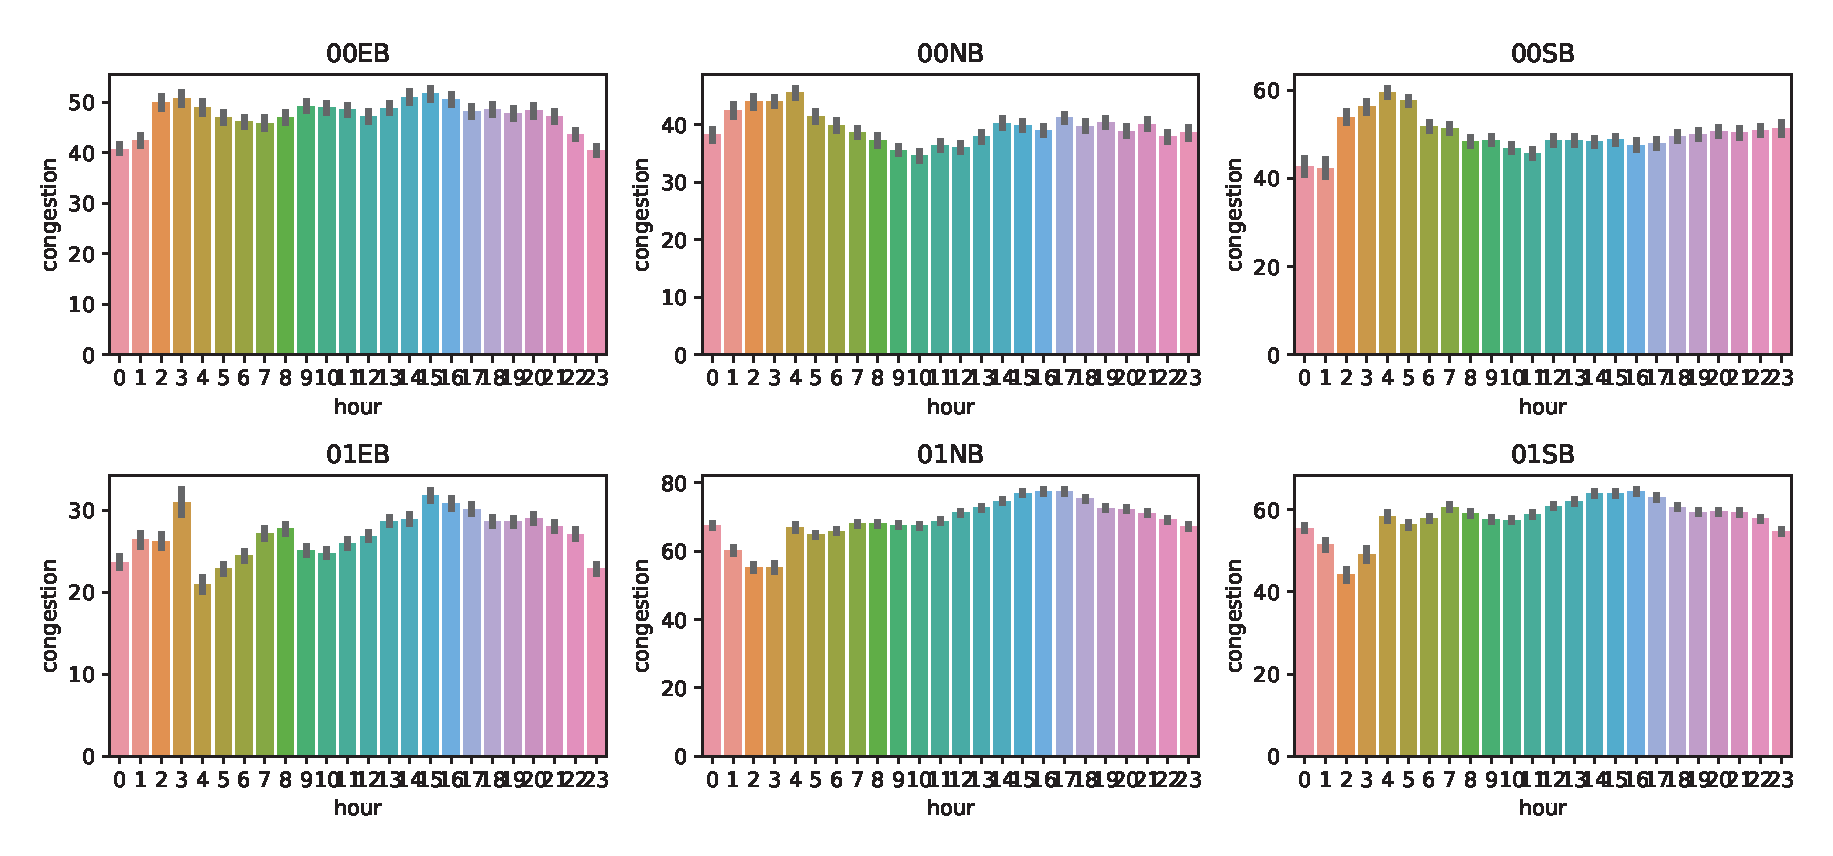
\includegraphics[width=10.0cm]{figure/road.eps}
		\centering
		\caption{The effect of hour on congestion group by road}
		\label{group by road}
\end{figure}

\begin{figure}
	
		\setlength{\abovecaptionskip}{0.1cm} 
		\raggedleft
		\includegraphics[width=10.0cm]{figure/hour.eps}
		\centering
		\caption{The effect of weekday on congestion group by hour}
		\label{group by hour}
\end{figure}

\begin{center}
	\begin{figure}
			\setlength{\abovecaptionskip}{0.1cm} 
			\raggedleft
			\includegraphics[width=10.0cm]{figure/period.eps}
			\centering
			\caption{The effect of period on congestion}
			\label{period}
	\end{figure}
\end{center}

\section{Model Train and Evaluation} \label{sec-experiment}
Before training the model, we carried out the following steps:\par
\begin{enumerate}
	\item Divide the training and validation sets using sklearn's library.
	\item Process the non-integer data from the training set, validation set and test set
\end{enumerate}\par
In this paper, a lightgbm model is used to train to predict congestion in the US metropolitan area with the following parameter settings:\par
'objective' : 'regression'\par
'metric': 'mae'\par
'learning_rate': 0.25\par
'num_iteration': 200\par
'num_leaves':250\par
'device':'gpu'\par
After setting up the model parameters, we encapsulated the data into the format required by lightgbm for training.\par
As the training was completed, we extracted the following features.(figure 10)\par
\begin{figure}[h]
	\includegraphics[width=8cm]{figure/feature_importance.eps}
	\caption{Feature Importance}
\end{figure}\par
In the evaluation phase of the model, we evaluated the model using the regression model evaluation metrics. The evaluation indicators are listed in the table 3 below:\par
\begin{table}[htb]
	\setlength{\abovecaptionskip}{0pt}
	\setlength{\belowcaptionskip}{10pt}
	\centering
	\caption{Model evaluation indexes}
	
	\begin{tabular}{ c | c  }
		\toprule
		Index    &  Eexplication \\
		\midrule
		explained_variance_score     &  \makecell{Explain the variance score of \\the regression model. }   \\
		mean_absolute_error		  &  \makecell{Assess the proximity of the predicted results to\\the real data set.} \\
		Mean squared error				  &  \makecell{Calculate the mean value of the square sum of the errors\\ of the corresponding sample points of the \\fitting data and the original data} \\
		r2_score				  			 &   \makecell{Judge the fitting degree of prediction model and real data} \\
		\bottomrule
	\end{tabular}
\end{table}
Three of these indicators were used for the assessment,the results of the assessment are as follows:\par
\begin{table}[htb]
	\setlength{\belowcaptionskip}{10pt}
	\caption{The Evaluation results}
	\begin{tabular}{c|c}
		\hline
		Index & Result  \\
		\hline
		explained_variance_score   & 0.7277243544483329    \\
		mean_absolute_error&  6.167491947603395 \\
		r2_score & 0.7277251135484366  \\
		\hline
	\end{tabular}
\end{table}\par
From Table 4, it can be seen that both explained_variance_score and r2_score are 0.73, so the model is well trained without optimization.

\section{Result} \label{sec-conclusions}
Based on the data from the test set, some of the test results are shown in the table 5 below:\par
\begin{table}[htb]
	\setlength{\abovecaptionskip}{10pt}
	\setlength{\belowcaptionskip}{15pt}
	\centering
	\caption{The prediction results}
	
	\begin{tabular}{p{2.5cm}p{2.5cm}p{2.5cm}p{2.5cm}}
		\hline
		Row_id & Congestion  &  Row_id & Congestion \\
		\hline
		848835 & 47 & 848836 & 33\\
		848837 & 39 & 848838 & 54\\
		848839 & 64 & 848840 & 23\\
		848841 & 28 & 848842 & 70\\
		848843 & 25 & 848844 & 47\\
		848845 & 46 & 848846 & 25\\
		848847 & 69 & 848848 & 60\\
		\hline
	\end{tabular}
\end{table}




